\section{Simulação de Experimentos Aleatórios em R}

A simulação computacional permite reproduzir experimentos aleatórios cujo
resultado não pode ser previsto com certeza. Na Ciência da Computação, em que a
probabilidade é indispensável, a simulação é um recurso importante na avaliação
do desempenho de sistemas \cite{harcholbalter2024probability} e também no
tratamento de problemas em que os dados dependem de um modelo
probabilístico \cite{chan2021probability}. Nesta seção, as funções
\textit{runif()}, \textit{sample()} e \textit{replicate()} são usadas para simular,
respectivamente, uma moeda, uma urna e a soma de dois dados, comparando as
frequências empíricas com as probabilidades teóricas. Ao final, a soma de dois
dados também ilustra a convergência da média amostral à medida que o número de
repetições aumenta.

A frequência relativa de um evento $A$, observado em $n$ repetições de um
experimento aleatório, é definida como a razão apresentada na
Equação~\ref{eq:freq}.

\begin{equation}
	f_n(A) = \frac{n_A}{n}
	\label{eq:freq}
\end{equation}

Na Equação~\ref{eq:freq}, $n_A$ conta quantas vezes o evento $A$ ocorreu nas $n$
repetições. Sob a interpretação frequentista, a probabilidade teórica $P(A)$
corresponde ao valor para o qual a frequência relativa converge quando o número
de repetições cresce, o que se denota por
$P(A) = \lim_{n \to \infty} f_n(A)$. Esse comportamento é garantido pela Lei dos
Grandes Números e é o que permite estimar
probabilidades por meio de simulação \cite{ross2010probabilidade}.

\subsection{Moeda e a convergência da frequência relativa}

Para simular uma moeda honesta, foram gerados $n = 5000$ números aleatórios
uniformes em $[0,1]$ com a função \textit{runif()}, contando como ``cara'' cada
valor menor que $0{,}5$. Como a probabilidade de um número uniforme cair abaixo de
$0{,}5$ é exatamente $0{,}5$, esse procedimento reproduz uma moeda honesta com
$P(\text{cara}) = 0{,}5$. Cada lançamento equivale a uma variável aleatória de
Bernoulli $X_i$, que assume o valor $1$ para cara e $0$ caso contrário. Como $X_i$
é uma variável indicadora e os lançamentos são independentes e identicamente
distribuídos \cite{harcholbalter2024probability}, a frequência relativa de caras
após $n$ lançamentos coincide com a média amostral dessas variáveis, definida na
Equação~\ref{eq:media_bernoulli}.

\begin{equation}
	\bar{X}_n = \frac{1}{n} \sum_{i=1}^{n} X_i
	\label{eq:media_bernoulli}
\end{equation}

Pela Lei dos Grandes Números, a média amostral $\bar{X}_n$ converge para o valor
esperado $E[X_i] = p = 0{,}5$ quando $n$ cresce \cite{ross2010probabilidade}. O
Listing~\ref{lst:moeda} gera os números uniformes e acompanha a frequência
relativa acumulada de cara.

\begin{lstlisting}[caption={Moeda simulada com \textit{runif()} e frequência relativa acumulada.}, label={lst:moeda}]
n_moeda <- 5000
result <- runif(n_moeda)
eh_cara <- result < 0.5
freq_rel <- cumsum(eh_cara) / seq_len(n_moeda)
\end{lstlisting}

A convergência dessa frequência aparece na Figura~\ref{fig:moeda}. Apesar da
forte oscilação inicial, a frequência relativa se estabiliza em torno do valor
teórico $0{,}5$ conforme $n$ cresce. A frequência relativa final observada foi
$0{,}4948$, com desvio de $0{,}0052$ em relação ao valor teórico.

\begin{figure}[H]
	\centering
	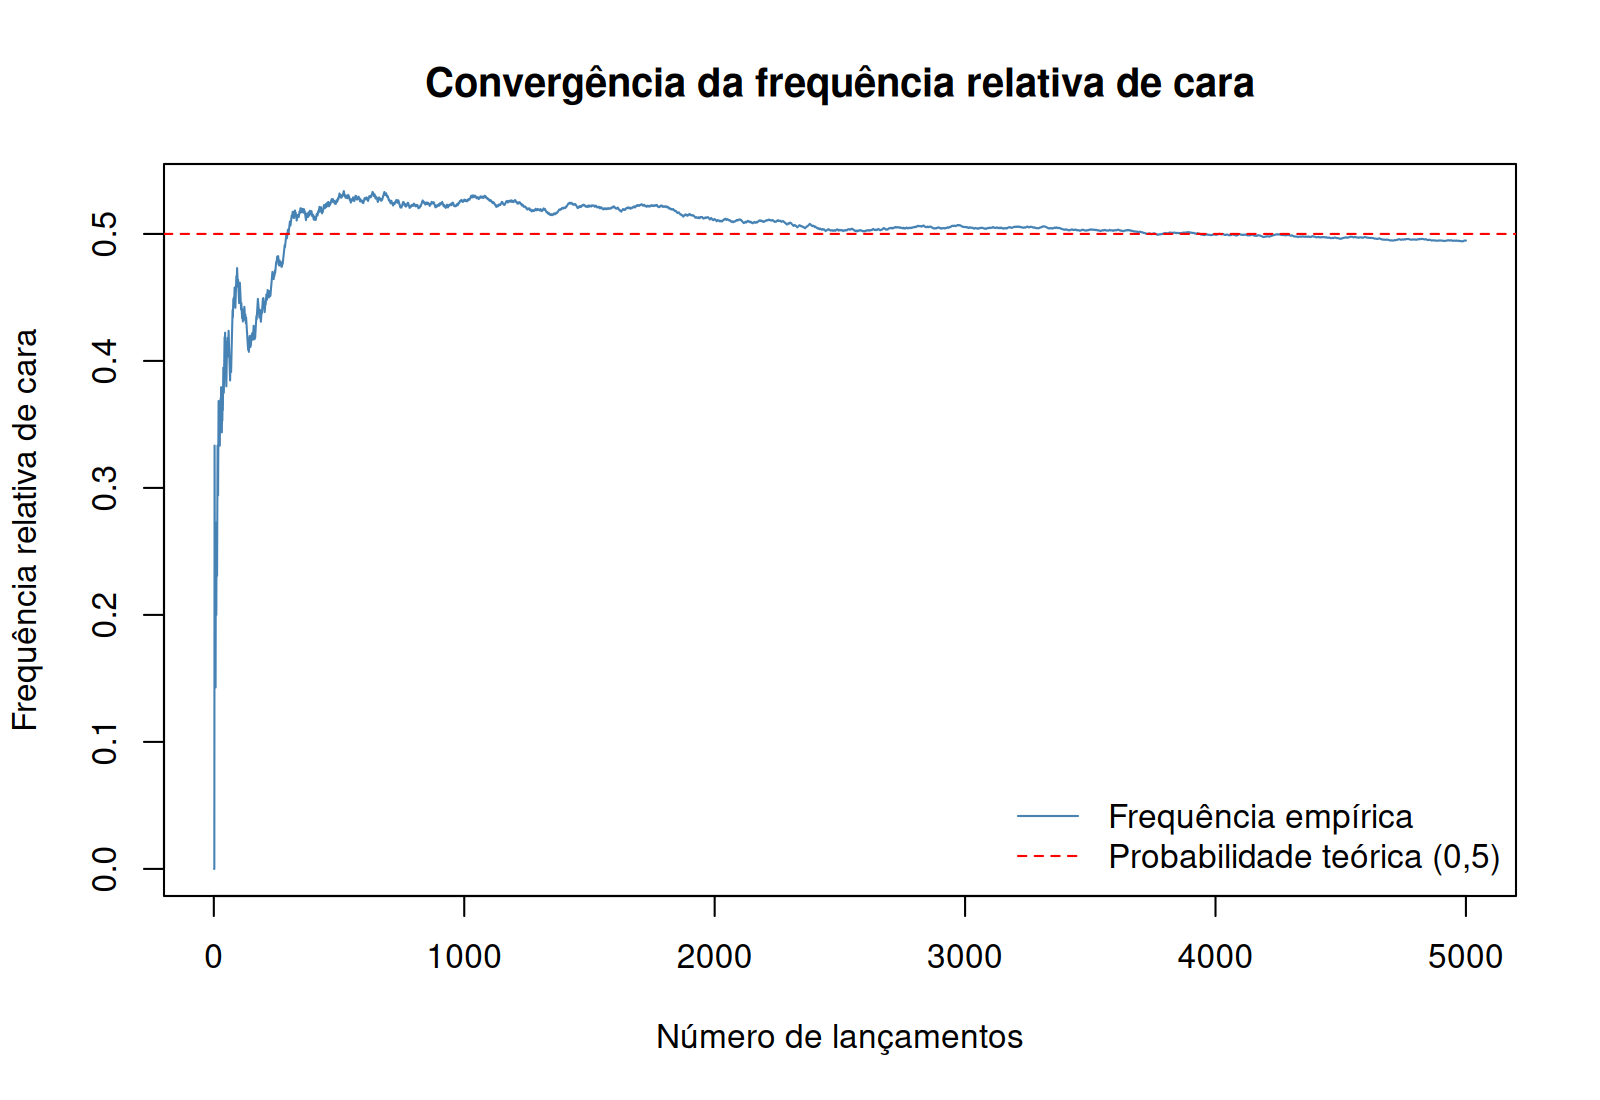
\includegraphics[width=0.8\textwidth]{secoes/02_simulacao/imagens/fig_moeda_convergencia.png}
	\caption{Convergência da frequência relativa de ``cara'' para $0{,}5$.}
	\label{fig:moeda}
\end{figure}

\subsection{Urna e a amostragem aleatória}

É considerada uma urna com 10 bolas, sendo 5 vermelhas, 3 azuis e 2 verdes. A
probabilidade de retirar uma bola de determinada cor é obtida pela razão entre o
número de bolas daquela cor e o total de bolas na urna, conforme a
Equação~\ref{eq:prob_urna}.

\begin{equation}
	P(\text{cor}) = \frac{\text{número de bolas da cor}}{\text{número total de bolas}}
	\label{eq:prob_urna}
\end{equation}

Pela Equação~\ref{eq:prob_urna}, as probabilidades teóricas de retirar cada cor
são, respectivamente, $5/10 = 0{,}5$, $3/10 = 0{,}3$ e $2/10 = 0{,}2$. Como cada
retirada é feita com reposição, o experimento é repetido sob condições idênticas
e de forma independente, de modo que as frequências relativas observadas estimam
as probabilidades teóricas \cite{ross2010probabilidade}. O Listing~\ref{lst:urna}
sorteia $n = 8000$ retiradas com a função \textit{sample()}.

\begin{lstlisting}[caption={Retiradas de uma urna com \textit{sample()}.}, label={lst:urna}]
urna <- c(rep("vermelha", 5), rep("azul", 3), rep("verde", 2))
n_urna <- 8000
retiradas <- sample(urna, size = n_urna, replace = TRUE)

freq_emp_urna <- table(factor(retiradas, levels = c("vermelha", "azul", "verde"))) / n_urna
prob_teo_urna <- c(0.5, 0.3, 0.2)
\end{lstlisting}

Os resultados aparecem na Figura~\ref{fig:urna}. As frequências observadas foram
$0{,}4984$ para vermelha, $0{,}2940$ para azul e $0{,}2076$ para verde, próximas
da composição real da urna, com desvio máximo de cerca de $0{,}008$ em relação
aos valores teóricos.

\begin{figure}[H]
	\centering
	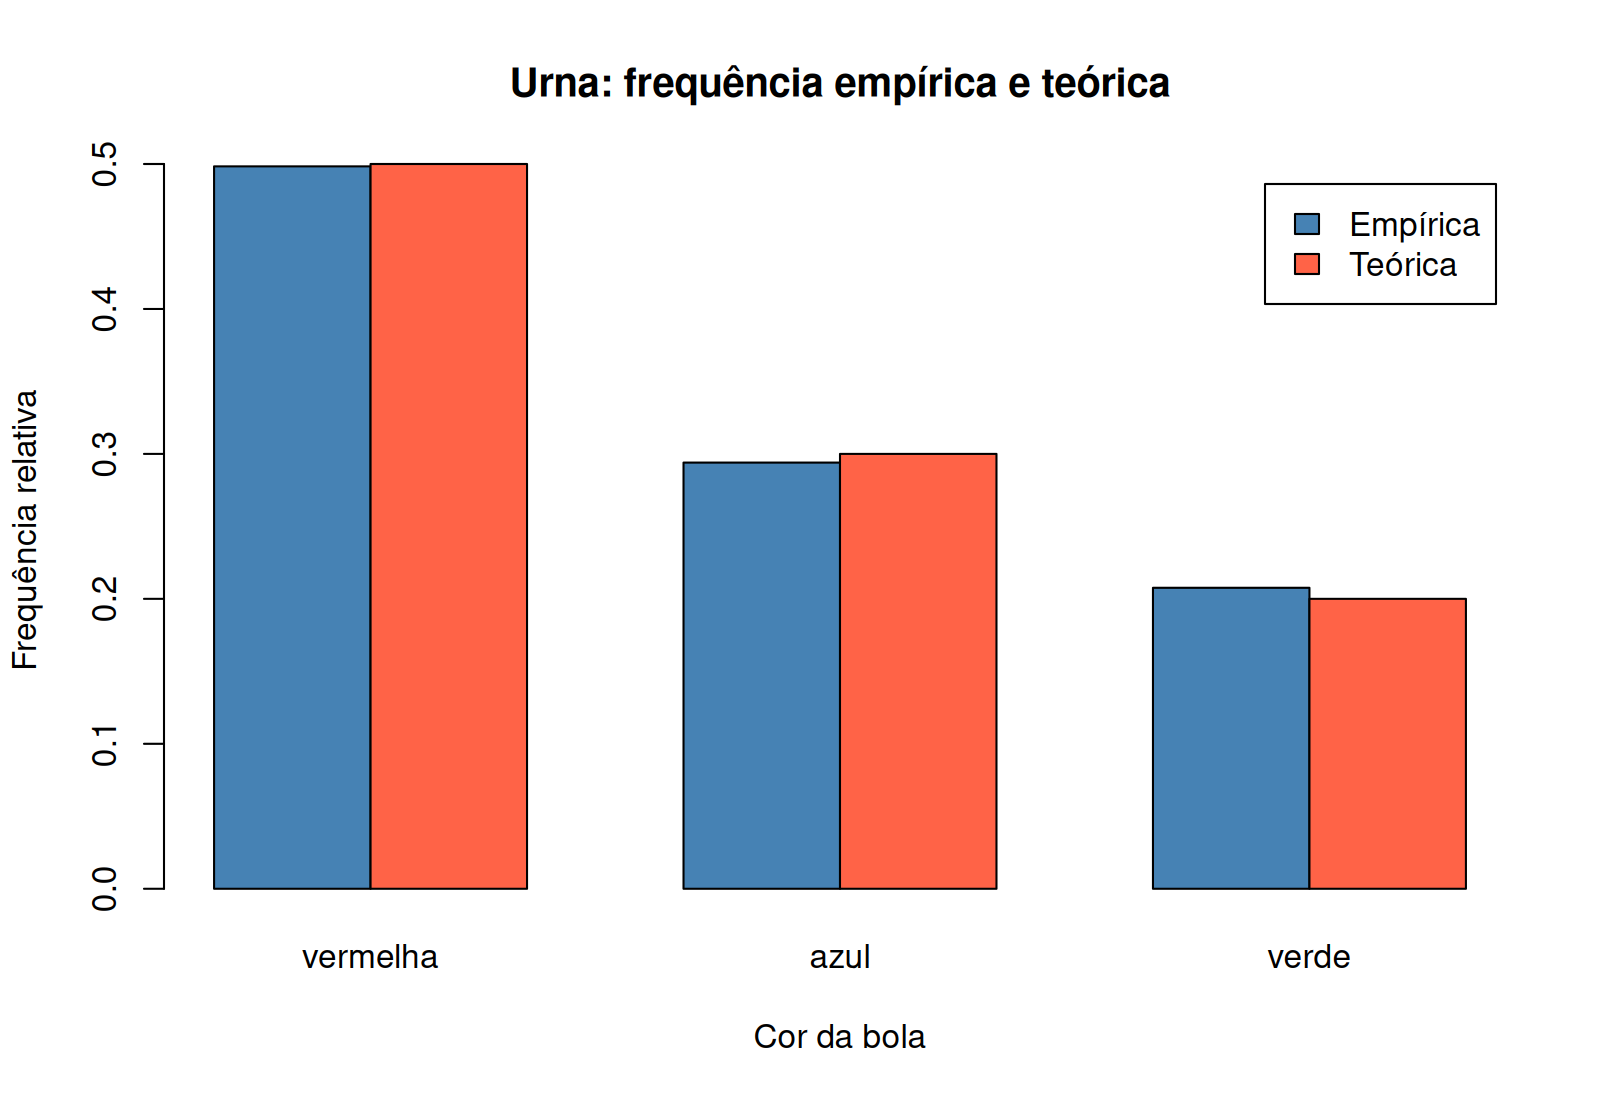
\includegraphics[width=0.8\textwidth]{secoes/02_simulacao/imagens/fig_urna_freq.png}
	\caption{Frequências empírica e teórica das cores da urna.}
	\label{fig:urna}
\end{figure}

\subsection{Soma de dois dados e a média amostral}

A função \textit{replicate()} permite repetir um experimento um número grande de
vezes. Aqui, o experimento consiste em somar dois dados honestos, repetido
$n = 20000$ vezes. A soma $S = X_1 + X_2$ pode assumir os valores inteiros de $2$
a $12$. Como os dois dados são lançados de forma independente e cada um tem seis
faces, existem $6 \times 6 = 36$ pares ordenados igualmente prováveis, e a
probabilidade de uma soma $s$ é a razão entre o número de pares que a produzem e o
total de $36$, conforme a Equação~\ref{eq:prob_soma}.

\begin{equation}
	P(S = s) = \frac{N(s)}{36}, \qquad N(s) = 6 - |s - 7|, \qquad s = 2, 3, \ldots, 12
	\label{eq:prob_soma}
\end{equation}

Na Equação~\ref{eq:prob_soma}, $N(s)$ é o número de pares $(i, j)$ com
$i + j = s$. Esse número cresce de $1$, para a soma $2$, até o máximo de $6$, para
a soma $7$, e decresce de forma simétrica até $1$, para a soma $12$, o que dá à
distribuição o formato triangular e torna a soma $7$ a mais provável
\cite{ross2010probabilidade}. O Listing~\ref{lst:soma} repete o experimento com
\textit{replicate()}.

\begin{lstlisting}[caption={Distribuição da soma de dois dados com \textit{replicate()}.}, label={lst:soma}]
n_rep <- 20000
soma <- replicate(n_rep, sum(sample(1:6, size = 2, replace = TRUE)))

freq_emp_soma <- table(factor(soma, levels = 2:12)) / n_rep
freq_teo_soma <- c(1, 2, 3, 4, 5, 6, 5, 4, 3, 2, 1) / 36
\end{lstlisting}

A distribuição obtida aparece na Figura~\ref{fig:soma}, que reproduz o formato
triangular esperado, com a soma $7$ sendo a mais frequente.

\begin{figure}[H]
	\centering
	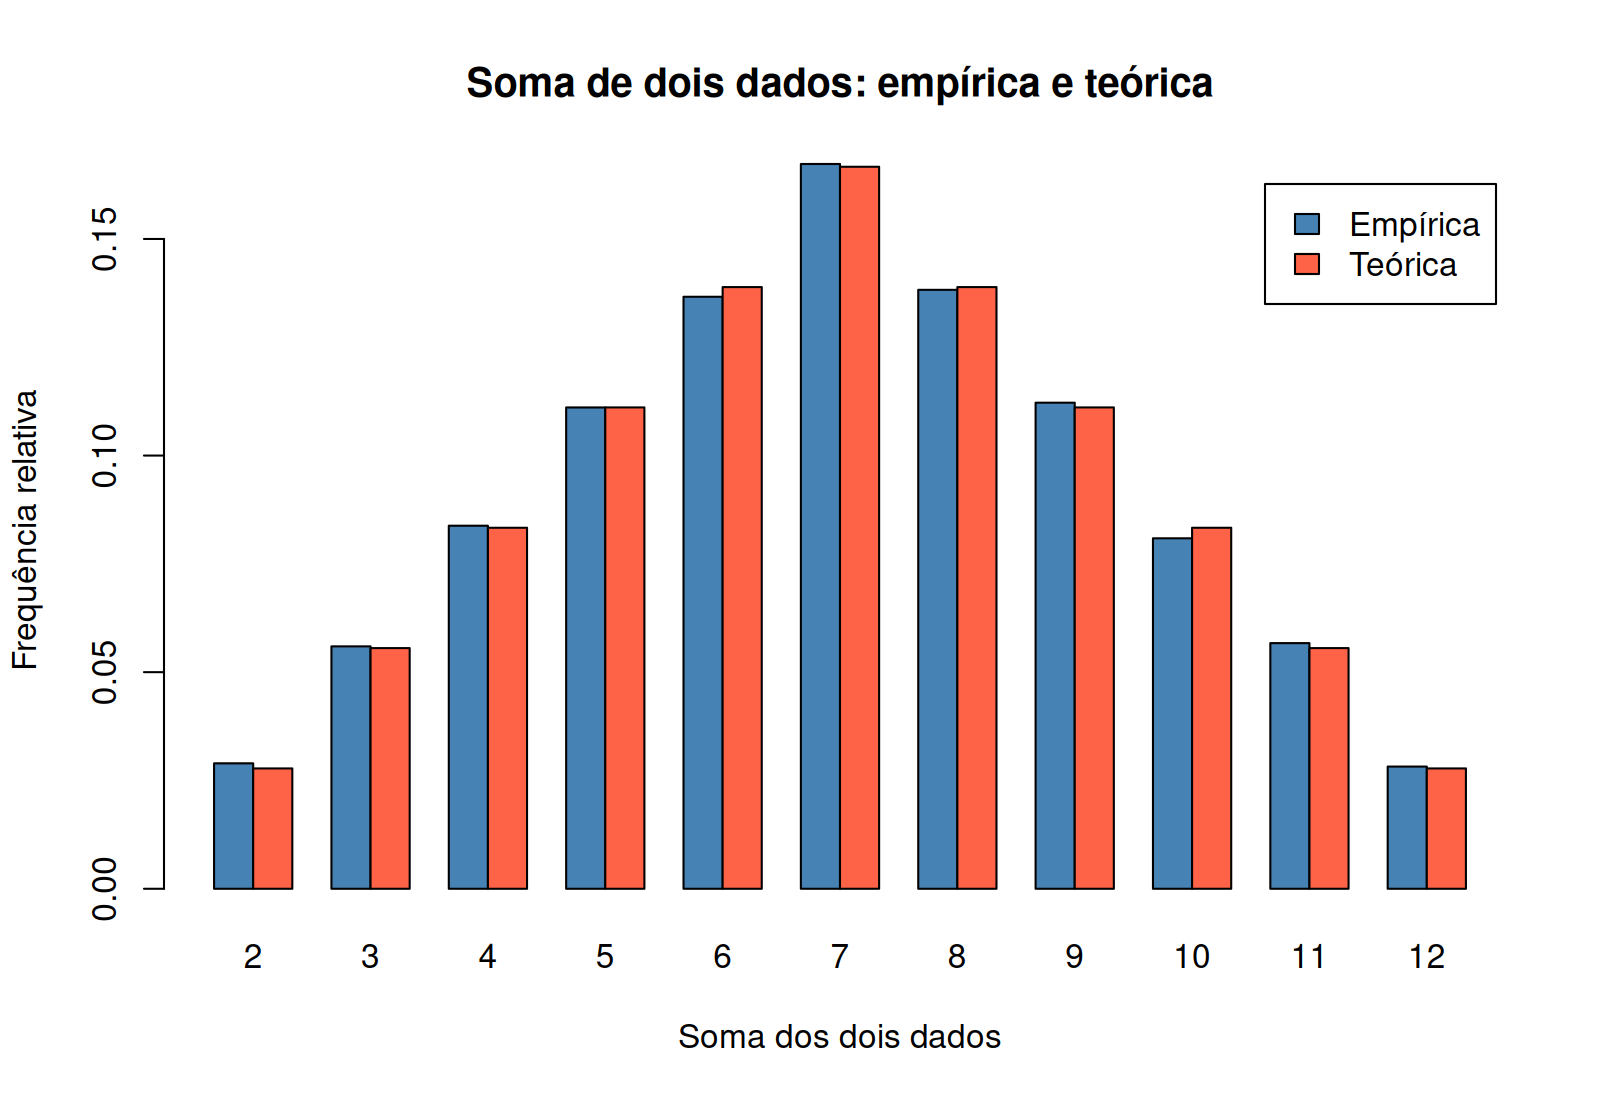
\includegraphics[width=0.8\textwidth]{secoes/02_simulacao/imagens/fig_soma_dois_dados.png}
	\caption{Distribuição empírica e teórica da soma de dois dados.}
	\label{fig:soma}
\end{figure}

A mesma simulação ilustra a convergência da média amostral, da qual a frequência
relativa da moeda é um caso particular. O valor esperado da soma é a soma dos
valores esperados de cada dado, conforme a Equação~\ref{eq:esperanca_soma}.

\begin{equation}
	E[S] = E[X_1] + E[X_2] = 3{,}5 + 3{,}5 = 7
	\label{eq:esperanca_soma}
\end{equation}

Pela Lei dos Grandes Números, a média acumulada das somas converge para
$E[S] = 7$ à medida que o número de repetições aumenta
\cite{ross2010probabilidade}. O Listing~\ref{lst:soma_media} acompanha essa média
acumulada.

\begin{lstlisting}[caption={Média amostral acumulada da soma de dois dados.}, label={lst:soma_media}]
media_soma <- cumsum(soma) / seq_len(n_rep)
\end{lstlisting}

A convergência é exibida na Figura~\ref{fig:soma_media}. A média amostral final
observada foi $6{,}9944$, próxima de $7$. A média acumulada oscila de forma
acentuada nas primeiras repetições e passa a se estabilizar em torno do valor
esperado, com flutuações que diminuem à medida que a amostra cresce.

\begin{figure}[H]
	\centering
	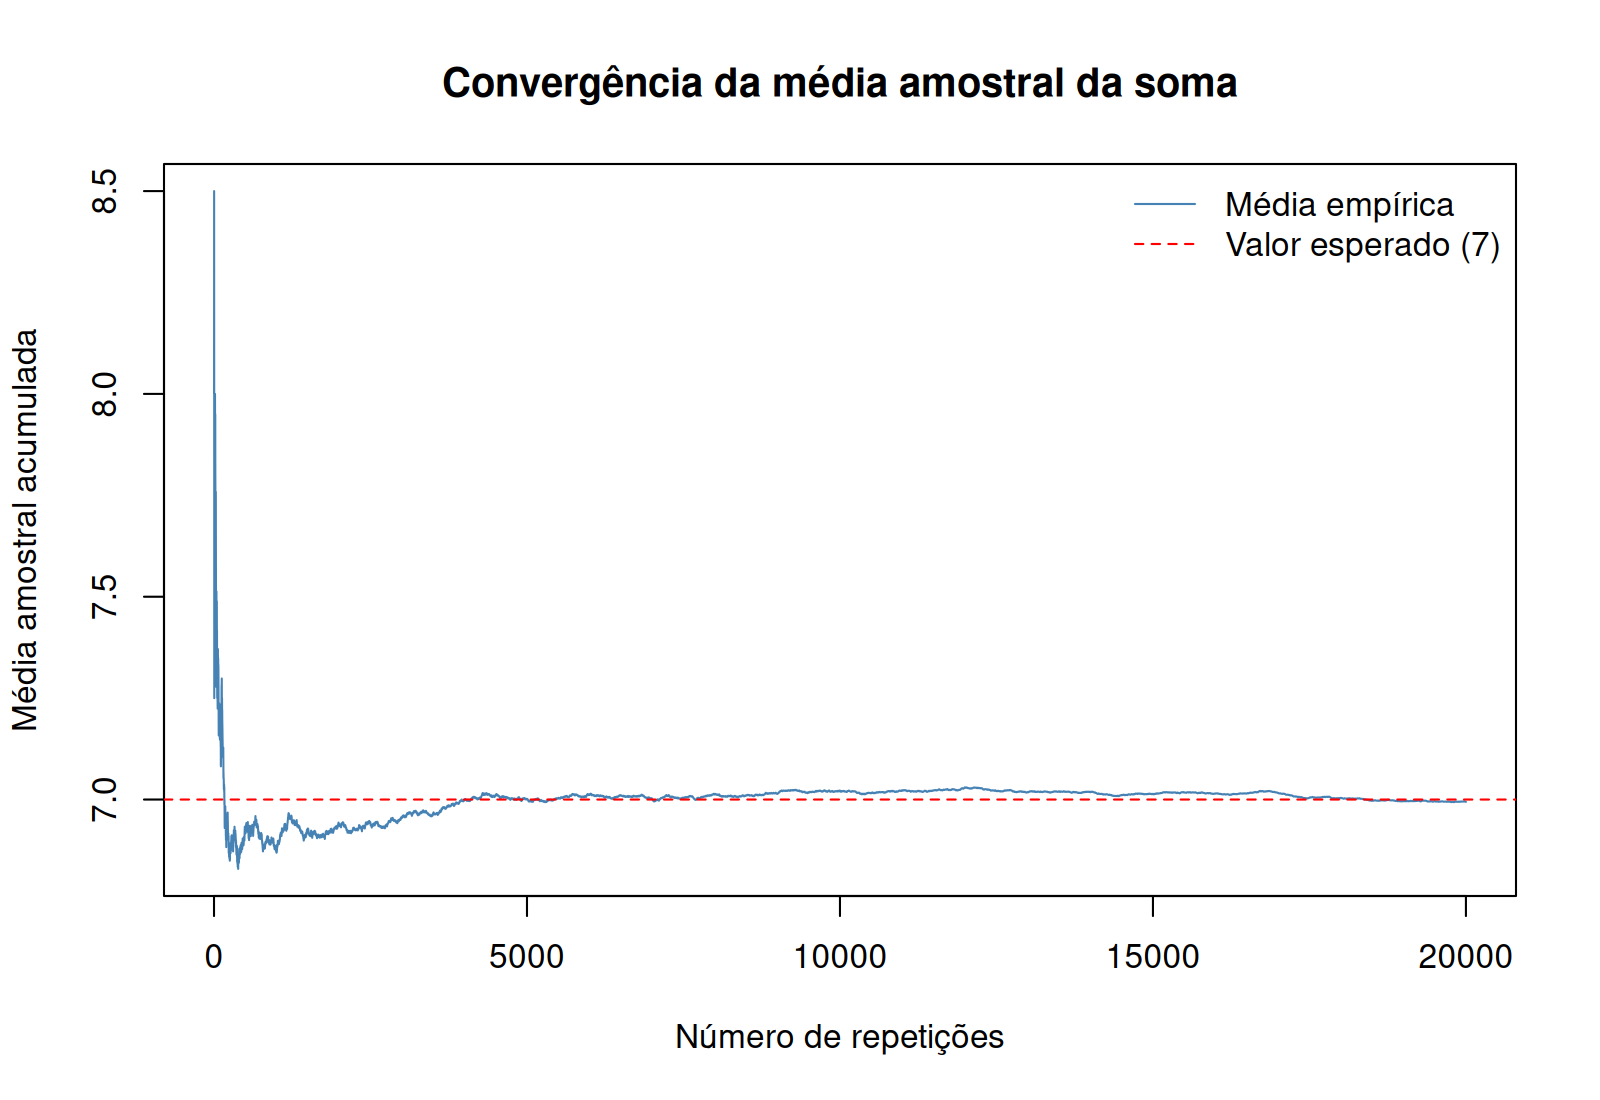
\includegraphics[width=0.8\textwidth]{secoes/02_simulacao/imagens/fig_soma_media.png}
	\caption{Convergência da média amostral da soma para $7$.}
	\label{fig:soma_media}
\end{figure}
